% #############################################################################
% This is Chapter 3
% !TEX root = ../main.tex
% #############################################################################
\fancychapter{Hybrid models for children automatic speech recognition}
\label{chap:Chapter3}
\cleardoublepage
%\section{Introduction}

% \ac{HMM-DNN} played a signifant role in \ac{ASR} (quick history recap)
In the history of \ac{ASR}, \ac{HMM}-based models emerged as a popular choice for acoustic modelling since the 1980s. The application of \acp{HMM} offered a structured framework to effectively model the temporal dependencies inherent in speech signals. Initially, the paradigm involved combining \acp{HMM} with \acp{GMM} to represent the probability distributions of acoustic features. This traditional \ac{HMM-GMM} architecture, while effective, faced limitations in capturing the intricacies of complex, non-linear relationships present in speech data. Therefore, a pivotal turning point occurred with the integration of \ac{DNN}, evolving towards hybrid \ac{HMM-DNN} models. This paradigm shift led to substantial improvements in \ac{ASR} performances. Indeed, \acp{DNN} brought enhanced modelling capabilities, allowing the system to discern more nuanced acoustic patterns and adapt better to diverse linguistic contexts. The hybrid \ac{HMM-DNN} approach has become key architecture in modern \ac{ASR} systems, demonstrating remarkable success in handling large vocabulary tasks and challenging acoustic conditions \cite{hmm-dnn}. 

% Why \ac{HMM-DNN} for children
In Chapter \ref{chap:Chapter2}, we explained the integration of acoustic, phonetic, and linguistic knowledge within the \ac{ASR} pipeline, particularly in the context of \ac{HMM-GMM} and \ac{HMM-DNN} systems. This integration includes the cooperation of multiple modules, such as the vocabulary, acoustic model, and language model, which all work together to support the Decoder's operations. By directly integrating hand-crafted knowledge into the \ac{ASR} system, the quantity of speech data needed to produce suitable results can be decreased. These characteristics were proven to be beneficial for children \ac{ASR} where the amount of data is often limited. For years, \ac{HMM}-based configurations have been a prominent choice in children's \ac{ASR} research. Between 2009 and 2020, a literature review \cite{big_review_childASR} found that 80\% of published research on children's speech recognition was based on \ac{HMM} systems, with 45\% using \ac{HMM-GMM} and 35\% \ac{HMM-DNN}. The literature suggests that \ac{ASR} results can be improved through the application of inductive bias approaches such as transfer learning and multi-task learning \cite{TransferLF}. However, a literature review \cite{big_review_childASR} showed that during the same period, 63\% of published work focused on English. Therefore, it remains uncertain how children's speech from other languages relates to the various approaches used in English, particularly transfer and multi-task learning.

% What we planned to do here
In this chapter, we aim to answer to the following research questions: \textit{Which knowledge transfer approach is best for efficiently modelling and improving traditional automatic recognition of children's speech? Can these approaches be used to efficiently exploit low-resource children's speech data from multiple languages?}. To this end, we will first present the \ac{TDNN-F} architecture used for the development of our \ac{HMM-DNN} \ac{ASR} system. Then, we will delve into applying knowledge transfer strategies across various scenarios, encompassing both non-English and English datasets. Applying it to the non-English dataset will allow us to understand if inductive bias approaches are still working in the context of non-English children's speech. To this end, we present an examination of both transfer and multi-task learning methodologies, leveraging adult speech as an inductive bias, a prevalent approach in the existing literature. 

Finally, as part of our contribution, we introduce a novel approach called ``multilingual transfer learning". This strategy integrates both transfer and multi-task learning techniques. Here, we address the challenge posed by the scarcity of data for both adults and children in low-resource languages by employing a combination of transfer and multi-task learning methodologies solely on low-resourced children's speech datasets.

\section{Factorised Time Delay Neural Network for children ASR}
\label{sec:TDNNF}
\begin{figure}[ht]
    \centering
    \subfigure[TDNN with sub-sampling]{\label{fig:tdnn}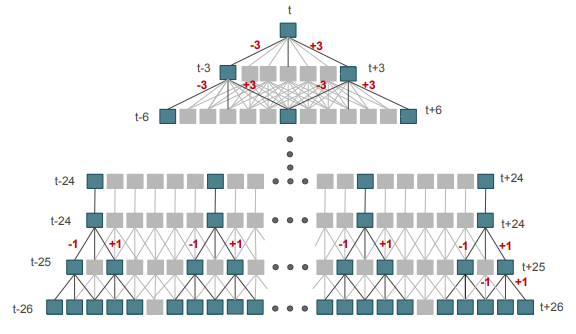
\includegraphics[width=0.49\textwidth]{imgs/TDNN.png}}
    \subfigure[Factorised TDNN layer]{\label{fig:tdnnf}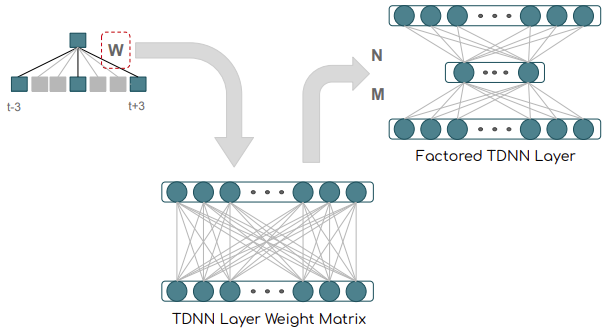
\includegraphics[width=0.49\textwidth]{imgs/TDNNF.png}}
    \caption{TDDN and TDNN-F taken from \cite{tdnnf-children}}
\end{figure}
% Focus on this section
In this chapter, we will focus on the application of \ac{HMM-DNN}-based models, specifically leveraging the \ac{TDNN-F} architecture.  Instead of revisiting the entire \ac{HMM-DNN} framework, extensively covered in Chapter \ref{chap:Chapter2}, we will delve into the distinctive features of the \ac{DNN} architecture employed in our \ac{HMM-DNN} \ac{ASR} systems, namely the \ac{TDNN-F}. 
The use of the particular \ac{TDNN-F} architecture instead of \acp{DNN} or \ac{TDNN} was motivated by the need to improve \ac{ASR} performances in scenarios characterised by limited speech data and its successful results for children \ac{ASR} \cite{tdnnf-children}. This choice aligns with the broader trend in \ac{ASR} research where there is increasing interest in exploring more data-efficient neural network architectures, with the \ac{TDNN-F} standing out as a notable example.

% How TDNN works
In a \ac{TDNN} layer, the input at time step $t$ is sent to the next layer along with its neighbouring frames within a specific context window \cite{tdnn}. The multiple  \ac{TDNN} layers enable the integration of information over a broader context window. However, this design can lead to computational inefficiency due to the overlap of adjacent steps context windows. In response to this computational issue, an alternative approach involves sub-sampling the input sequence, skipping certain frames and transmitting only the sampled frames. This sub-sampling process is illustrated in Figure \ref{fig:tdnn}. 
The sub-sampling technique offers a trade-off between computational efficiency and the network's ability to capture temporal dependencies. This is based on the assumption that neighbouring activations are correlated. Therefore, by selectively processing a subset of frames, the TDNN can maintain its ability to capture relevant information while reducing the computational cost associated with processing every frame.

% How TDNN-F works
The \ac{TDNN-F} architecture \cite{TDNN-F} enhances the \ac{TDNN} by improving the computational efficiency of the network. This is achieved by decomposing the weight matrix of each \ac{TDNN} layer into an approximation as the product of two lower-rank matrices using \ac{SVD}, defined as:
\begin{equation}
    \text{W} = \text{U}\Sigma \text{V}^T = \text{MN}
\end{equation}
Here, $\Sigma \in \mathbb{R}^{m \times n}$ is a non-negative rectangular diagonal matrix, and $\text{M} \in \mathbb{R}^{m \times k}$ and $\text{N} \in \mathbb{R}^{k \times n}$ with $k \leq \min(m,n)$. The goal is to ensure that one of the two sub-matrices is close to a semi-orthogonal matrix, representing either $\text{U}\Sigma$ or $\Sigma \text{V}^T$. Notably, $k$ is typically chosen to be much smaller than $m$ and $n$.
During the training of the network, after every few updates of the entire network, a specific update is performed on matrix $\text{N}$ using \ac{SGD}. This update is guided by an additional objective function, which ensures that $\text{N}$ is not too far from being semi-orthogonal.
The introduction of the semi-orthogonal constraint through the matrix factorisation process in \ac{TDNN-F} can be viewed as adding an extra ``bottleneck layer" to the traditional \ac{TDNN}. A visual representation of the \ac{TDNN-F} layers is presented in Figure \ref{fig:tdnnf}. This ``bottleneck layer", represented by the reduced-rank matrix $\text{N}$, contributes to the overall efficiency of the network by reducing the number of parameters and computations required while preserving essential information.

\section{Assessing the efficacy of multi-task and transfer learning from adult to children}
\label{section:HMMDNNADULT2CHILD}
\subsection{Methodology}

% Motivation
Using adult data as an inductive bias for knowledge transfer approaches in children's ASR has been found to be beneficial in tackling the challenges specific to children's ASR, as highlighted in the literature \cite{TFchildren,TransferLF,2019multi}. The motivation behind leveraging adult data for pre-training lies in the stability and reduced variability found in adult speech. This characteristic simplifies the extraction and recognition of intrinsic and meaningful speech patterns, making it an efficient approach for knowledge transfer to improve children's \ac{ASR}. In this initial experiment, our aim is to first validate these findings and subsequently extend these methods to a low-resource language. To this end, we propose to assess children's speech recognition performances in four distinct configurations:

%Motivated by the success of knowledge transfer approaches for children's \ac{ASR} using adult data as inductive bias in the literature \cite{TFchildren,TransferLF,2019multi}, we aim to extend and validate these findings using both a low-resource language and English. The reason for leveraging adult data for pre-training lies in the stability and reduced variability found in adult speech. This characteristic simplifies the extraction and recognition of intrinsic and meaningful speech patterns that can be efficiently used for knowledge transfer. Therefore, we propose to assess children's speech recognition performances in four distinct configurations:


\begin{enumerate}
    \item \textbf{Adult model}: Training a model from scratch using only adult data. This configuration serves as a baseline to assess the standalone performance of a model trained exclusively on adult speech.
    \item \textbf{Children model}: Training a model from scratch using only children's data. This configuration provides insights into the model's ability to learn from children's speech without leveraging adult data.
    \item \textbf{Multi-task model}: Training a model concurrently on adult and children data using multi-task learning. This configuration explores the potential benefits of simultaneous training on both adult and children data.
    \item \textbf{Transfer learning}: Fine-tuning a model on children's data that was pre-trained on adult data (from the Adult Model in Configuration 1). This configuration assesses the effectiveness of transferring knowledge from adult to children data for improved speech recognition.
\end{enumerate}

By systematically comparing these configurations, our objective is to identify the most effective approach for enhancing performance in children \ac{ASR}, particularly in low-resource language scenarios.


\subsection{Corpus}
\label{sec:corpus}
For our evaluation of knowledge transfer performances in children's speech, we considered both English and a low-resource language, specifically European Portuguese. European Portuguese can be qualified as a low-resource language due to the limited availability of large-scale adult speech corpora, with most datasets not exceeding 100 hours \cite{tribus}.
In our experiments, we utilised a subset of the LibriSpeech corpus for English and the BD-PUBLICO corpus for Portuguese as the adult corpora. For the children's dataset, we employed Myst and LetsRead for English and Portuguese, respectively. In this section, we offer a description of the adult corpora. Detailed information on both children datasets can be found in Section  \ref{section:children_corpora}. The statistics of all corpora used in this initial experiment are presented in Table \ref{tab:statistics_exp1}.
%In our evaluation of children's speech performance in a low-resource language context, we have chosen European Portuguese as our target language. European Portuguese qualifies as a low-resource language due to the limited availability of large-scale adult speech corpora, with most datasets not exceeding 100 hours \cite{tribus}.
% For this experiment, we used the LetsRead child corpus, detailed in Section \ref{section:children_corpora}, to represent children's speech in European Portuguese. Additionally, we employed the BD-PUBLICO corpus as the adult counterpart. The statistics of both corpora are presented in Table \ref{tab:statistics_exp1}.

% Stat corpus 
%\begin{table}[h]
%\begin{center}
%\begin{tabular}{lcc}
%\hline
%Corpus name      & Train & Test  \\ \hline
%\multicolumn{1}{l}{BD-PUBLICO}             & 8085 utt  & 412 utt  \\ 
%\multicolumn{1}{c}{\textit{Adult}}              & 21h48 & 01h10 %\\\hline
%\multicolumn{1}{l}{LETSREAD}     & 3590 utt & 1039 utt \\ 
%\multicolumn{1}{c}{\textit{Children}}     & 12h00 & 02h30 \\  \hline
%\multicolumn{1}{l}{Librispeech}                     & 281241 utt &   \\ 
%\multicolumn{1}{l}{}      &                &  960h &  \\ \hline
%\end{tabular}
%\caption{Number of utterances and duration of the different corpora for multi-task and transfer learning experiments using adult and children data}
%\label{tab:statistics_exp1}
%\end{center}
%\end{table}

\begin{table}[h]
    \begin{center}

    \begin{tabular}{cccc}
    \hline
    Language                    & Corpus name                                                                  & Train             & Test            \\ \hline
    \multirow{6}{*}{English}    & \multirow{3}{*}{\begin{tabular}[c]{@{}c@{}}LibriSpeech\\ \textit{Adult}\end{tabular}} & 104014 utterances & 2620 utterances \\
                                &                                                                              & 2097 speakers     & 87 speakers     \\
                                &                                                                              & 363h              & 5h              \\ \cline{2-4} 
                                & \multirow{3}{*}{\begin{tabular}[c]{@{}c@{}}Myst\\ \textit{Children}\end{tabular}}     & 60897 utterances  & 4079 utterances \\
                                &                                                                              & 566 speakers      & 91 speakers     \\
                                &                                                                              & 113 hours         & 13 hours        \\ \hline
    \multirow{6}{*}{Portuguese} & \multirow{3}{*}{\begin{tabular}[c]{@{}c@{}}BD-PUBLICO\\ \textit{Adult}\end{tabular}}  & 8085 utterances   & 412 utterances  \\
                                &                                                                              & 100 speakers      & 10 speakers     \\
                                &                                                                              & 22 hours          & 1 hour          \\ \cline{2-4} 
                                & \multirow{3}{*}{\begin{tabular}[c]{@{}c@{}}LetRead\\ \textit{Children}\end{tabular}}  & 3590 utterances   & 1039 utterances \\
                                &                                                                              & 180 speakers      & 52 speakers     \\
                                &                                                                              & 12 hours          & 2 hours         \\ \hline
    \end{tabular}
    \caption{Number of utterances, number of speakers, and the duration of training and testing sets for both English and Portuguese corpora, encompassing both adult and children training and test sets}
\label{tab:statistics_exp1}
\end{center}

    \end{table}


\subsubsection*{LibriSpeech}
The LibriSpeech dataset \cite{librispeech} is a widely used English corpus in the \ac{ASR} field, introduced to address the need for large-scale, high-quality speech datasets to advance \ac{ASR} research. The dataset consists of diverse audio recordings derived from audiobooks obtained from the LibriVox project, totalling approximately 1000 hours of labelled audio sampled at 16 k\ac{Hz}. LibriVox, a community-driven initiative, involves volunteers reading and recording around 8,000 public domain books at the time of the creation of Librispeech. Thus, LibriSpeech encapsulates the natural variability present in real-world spoken language, featuring speakers from diverse backgrounds and reading styles.

LibriSpeech is organised into different subsets, with the training data split into three partitions of 100 hours, 360 hours, and 500 hours. The development and test data are categorised as ``clean" and ``other" respectively, based on the difficulty levels for \ac{ASR} systems. In our experiments, we used the 360-hour training set, as it already represents well-resourced scenario conditions.


\subsubsection*{BD-PUBLICO}
The BD-PUBLICO database (Base de Dados em Português eUropeu, vocaBulário Largo, Independente do orador e fala COntínua) \cite{bdpublico} consists of reading sentences extracted from the Portuguese newspaper PÚBLICO over a 6-month period, from the beginning of September 1995 until March 1996. Recordings involve 120 speakers, specifically graduate and undergraduate students from Instituto Superior Técnico (Lisbon), all falling within the age range of 19 to 28 years, establishing BD-PUBLICO as an adult dataset. Recordings occurred in optimal noise conditions within a soundproof room at INESC-ID (Lisbon), with a sampling frequency of 16kHz and the use of a high-quality microphone. The corpus includes a pronunciation lexicon with phonemic transcriptions, with manual corrections applied to enhance transcription accuracy.

For effective model training and evaluation, we partitioned the BD-PUBLICO corpus into three distinct sets, ensuring balanced gender distribution. The training set comprises 80 sentences performed by each of the 100 speakers. The development set, consisting of 40 sentences performed by 10 speakers. Finally, the test set includes 40 sentences performed by 10 speakers.


\subsection{Experimental setup}
\label{section:exp_setup}

All experiments were conducted using the Kaldi open-source toolkit \cite{kaldi}. Initially, for each corpus, an independent \ac{HMM-GMM} acoustic model was trained to generate the necessary alignment for the training of the \ac{HMM-DNN} model. Subsequently, \ac{HMM-DNN} acoustic models were trained using 40-dimensional \ac{fbanks} alongside 40-dimensional \ac{SSC} features \cite{ssc}. The incorporation of \ac{SSC} features, which share properties with formant frequencies, is expected to enhance vowel recognition and contribute to improved recognition of children's speech. The resulting 80-dimensional input features were augmented by a 100-dimensional speaker embedding i-vector. Concatenating speaker embeddings to the input features is a commonly employed strategy to enhance model speaker robustness \cite{ivector}. Our i-vector extractor was specifically trained on a pooled set of children's data, encompassing LetsRead, PfStar Swedish, Etltde, Cmu kids, and Chorec, all described in Section \ref{section:children_corpora}.

To augment the training corpora, data augmentation techniques were applied, including perturbing the speaking rate of each training utterance by factors of 0.9 and 1.1, as well as volume perturbation. This augmentation strategy enhances the network's robustness to variations in speaking rate and volume during testing. Additionally, Specaugment \cite{specaugment} was employed on top of the \ac{fbanks} and \ac{SSC} features, involving random masking of time and frequency bands to further improve model robustness.

For all experiments, the same \ac{HMM-DNN} acoustic model architecture was employed, trained using the \ac{LF-MMI} objective function in conjunction with a cross-entropy loss. The learning rate used for training was $2 \cdot 10^{-4}$. The acoustic model architecture is divided into two parts: i) six convolutional neural network layers and seven \ac{TDNN-F} layers with a dimension of 1024, followed by ii) two \ac{TDNN} layers with a dimension of 450 and a single fully-connected layer working as an output layer. In the transfer learning experiments, only the first part of the network was fine-tuned, while the second part was replaced by randomly initialised layers. Similarly, in \ac{MTL} experiments, the first part was shared between adult and child models, while the second part remained independent. 

\subsection{Results}

\begin{table}[h]
    \centering
    \begin{tabular}{c|cc|cc}
    \hline
                      & \multicolumn{2}{c}{\textit{English}} & \multicolumn{2}{|c}{\textit{Portuguese}} \\ \hline
    Method            & Adult WER  $\downarrow$  & Children WER $\downarrow$  & Adult WER  $\downarrow$   & Children WER  $\downarrow$   \\ \hline
    Adult model       & \textbf{6.53\%}      & 43.87\%       & \textbf{3.82\%}       & 102.83\%        \\
    Children model    & 15.78\%     & 25.53\%       & 45.56\%      & 25.88\%         \\
    Multi-task model  & 6.74\%      & 30.56\%       & 4.59\%       & 27.65\%         \\
    Transfer learning & -           & \textbf{21.53\%}       & -            & \textbf{25.36\%}         \\ \hline
    \end{tabular}
    \caption{WER results using adult data for knowledge transfer methods}
\label{tab:res_exp1}

    \end{table}

%\begin{table}[h]
%\centering
%\begin{tabular}{c|ccc}
%\hline
% Method & Adult WER $\downarrow$   & Children WER  $\downarrow$   \\ \hline
%\multicolumn{1}{c|}{Adult model} & 3.82\%   &  102.83\%\\ 
%\multicolumn{1}{c|}{Children model} & 45.56\%  & 26.88\% \\ 
%\multicolumn{1}{c|}{Multi-task model}  &   4.59\% &  27.65\% \\ 
%\multicolumn{1}{c|}{Transfer learning} &  -  & \textbf{25.36\%} \\ \hline
%\multicolumn{1}{c|}{Transfer learning from Librispeech} & -  & 25.18\% \\ \hline


%\end{tabular}

%\caption{WER results using adult data for knowledge transfer methods}
%\label{tab:res_exp1}
%\end{table}

% Adult model

The \ac{WER} scores for all settings are presented in Table \ref{tab:res_exp1}. In the first row, we observed that employing a model trained solely on adult data yields a \ac{WER} of 43.87\% and 102.83\% on the children's corpora for English and Portuguese, respectively. Meanwhile, the same adult model achieves \ac{WER} scores of 6.53\% and 3.82\% for Librispeech and BD-PUBLICO, respectively. The notable degradation in children's scores compared to adults demonstrates the considerable variability present in children's speech, which has a detrimental impact on the \ac{ASR} scores. We observed that the Portuguese children's score degradation is higher than the English one, which can be explained by the higher mismatch between the adult and children recording setting coupled with the youngest age range in the Portuguese dataset. This underscores the notion that a dedicated acoustic model tailored specifically for children is essential, as children's speech recognition underperforms on adult systems.
%This supports the idea that an acoustic model designed exclusively for children is necessary because child speech is currently unusable with adult systems.

% Children model
On the other hand, training the acoustic model directly on children's data yields substantial improvements of the \ac{WER} on the children's test sets, reaching 25.53\% and 26.88\% for English and Portuguese, respectively. This indicates that exposing the model to children's acoustic variabilities during training enhances its robustness to such variations. However, this improvement comes at the cost of deteriorated adult speech recognition performance, resulting in \ac{WER} of 15.78\% and 45.56\% for English and Portuguese corpora, respectively. This further confirms the presence of acoustic mismatch between adult and children's speech. Subsequently, we compare the \ac{TL} and \ac{MTL} approaches using these two models trained from scratch as a baseline.

% Multi-task
In the \ac{MTL} scenario, where the model is trained jointly using both adult and children data at the same time, recognition \ac{WER} scores for adults and children marginally decrease compared to their individual baseline counterparts. However, unlike the adult and children baseline models, where the acoustic mismatch significantly impacted the \ac{WER} scores on the mismatch domain, the \ac{MTL} scenario shows comparable recognition scores to their respective ``trained from scratch" baselines. The inclusion of corpus-specific layers in the acoustic model architecture plays a crucial role. The shared component learns key characteristics of speech, using both sources of information, while the corpus-specific part focuses on applying these characteristics to the specific characteristics of adults and children, respectively. We also observed that the score gap between the children-alone model and the children's score in the multi-task setting is higher in the English setup. This discrepancy can be attributed to the significantly unbalanced amount of training data in the adult corpus compared to the children's amount of training data. While the gap in the Portuguese setup is only around 10 hours, it reaches approximately 250 hours in the English setup. This observation highlights a limitation of the \ac{MTL} method, wherein a mismatch in corpus sizes can lead to biased representations. Emphasising the need for careful selection of the different datasets used in the multi-task methodology.
% TL BD-Publico

In the last line of Table \ref{tab:res_exp1}, we evaluated training the model on children data using as initialisation the pre-trained adult model, of the first row. This \ac{TL} enhanced the children's results to 21.53\% and 25.36\% \ac{WER} for the English and Portuguese respectively. This configuration emerged as the most effective in our experiments for both English and Portuguese children's \ac{ASR}. When compared to random initialisation, it is shown that the weights learned in the adult pre-trained model are a beneficial starting configuration and allow the \ac{TL} to use the learnt patterns to tackle children's speech. Indeed, this \ac{TL} approach avoids the need for the model to learn these patterns from scratch, which is particularly difficult when using data from a highly variable source like children's speech. As a result, transfer learning may be considered a viable strategy for improving the \ac{ASR} performance for children's speech. This finding is consistent with the literature on hybrid models\cite{TransferLF,TFchildren}. 


% Conclusion
In this study, we conducted a knowledge transfer techniques analysis to improve the results of \ac{ASR} systems for children in both English and European Portuguese. We corroborate the acoustic mismatch between adult and child speech and the importance of the model to be trained on children's speech data. Our investigations revealed that the \ac{TL} approach is a promising way to improve low-resource children's speech recognition scores. Furthermore, multi-task learning was found to be helpful in the setting of mixed adult-child \ac{ASR} acoustic modelling. 
% Open question for next section
However, in this study, our primary focus is on the transfer from adults to children. Therefore, the effectiveness of such systems trained using only children's data is not clear. Additionally, while both \ac{MTL} and \ac{TL} individually improved the model for children's \ac{ASR}, we would be interested in exploring the potential benefits of their combined use.


\section{Combining multi-task and transfer learning using multilingual children data}
\subsection{Motivation}
% Explain motivation
In this section, we present our contribution, where we investigate the potential improvement in the performance of children's \ac{ASR} for low-resourced languages by leveraging children's resources from various languages. Indeed, in many scenarios, both adult's and children's speech data are limited or even unavailable. To overcome the challenges posed by substantial acoustic variability and data scarcity, we propose a novel approach that uses several small-sized corpora of children from diverse languages. Our study extends conventional multilingual training and \ac{TL} techniques for hybrid \ac{HMM-DNN} \ac{ASR}. We combine these techniques in a meaningful way to use knowledge from heterogeneous data sources. Initially, a multilingual model is trained using a \ac{MTL} objective, aiming to optimise network parameters for the distinct characteristics of children's speech across multiple languages simultaneously. Subsequently, this trained multilingual model is employed to enhance \ac{ASR} performance for a target language. Note that the target language may be different from those included in the multilingual training stage. This is achieved through transfer learning, where the knowledge gained from the multilingual model is adapted to the specific characteristics of the target language.


\subsection{The Multilingual-transfer learning approach}
\label{section:method}

We propose a new approach that combines \ac{TL} and \ac{MTL} together for improved acoustic modelling of hybrid \ac{HMM-DNN} \ac{ASR}. The proposed approach consists of a two-stage procedure using both \ac{MTL} and \ac{TL} that extends the existing techniques since these are usually applied separately. First, a multilingual model trained with a \ac{MTL} objective aims to optimise specifically the shared part of the network to better model the particular characteristics of children's speech. This is done across multiple languages in parallel. In this work, the model is considered multilingual because all the tasks trained during \ac{MTL} involve corpora of children from different languages.
Secondly, we adapt this multilingual model for a specific children's corpus with \ac{TL}. The motivation for using \ac{TL} as a second stage is to take advantage of the robust pre-trained model trained during the \ac{MTL} phase. Indeed, this pre-trained model has potentially learned cross-linguistic information about children's speech but has also seen more children's data than a model trained in a single language. 
For this purpose, the acoustic model is divided into two parts: the layers close to the input are shared across all languages, and the top layers, near the output, are language-specific. In other words, there are as many output layers as there are languages, i.e., children corpora. It is worth noting that one can incorporate a new language/task in this second stage by adding a new language-specific output, even if this new language/task has not been seen during \ac{MTL} training (see Figure \ref{fig:MLTL1}).

Our hypothesis is that the more data from heterogeneous sources seen by the acoustic model in the \ac{MTL} phase, the better the shared layers could capture the underlying characteristics of children's speech. Then, these learned characteristics can be used effectively, later, by the language-specific layers and during the \ac{TL} step of the procedure (figure \ref{fig:MLTL1}). 

Although the \ac{MTL} and \ac{TL} approaches adopted in this work have been used previously in other studies \cite{TransferLF,2019multi}, where researchers successfully applied \ac{MTL} using children speaking Mandarin and English, obtaining a relative improvement of 16.96\% \ac{WER} in the English children case, it is clear that the successful performance of this approach in the case of English cannot be expected to generalise to other contexts and languages. Indeed, English is a large-size, resource-rich pluricentric language, which should be seen more as an exceptional case rather than an average representative. It is important to emphasise that there is a need for research that investigates whether these methods, which have already been tested for English, also work in new scenarios, such as low to medium-resource languages with fewer resources than English, like Dutch, Portuguese, Swedish, and German.


%Although the approaches adopted in this work have been used previously in other studies, for instance \cite{TransferLF} and \cite{2019multi} where they successfully applied \ac{MTL} using children speaking  Mandarin and English, obtaining a relative improvement of 16.96\% \ac{WER} in the English children case, it is clear that successful performance of this approach in the case of English cannot be expected to generalise to other contexts and languages.  
%Indeed, English is a large-size, resource-rich pluricentric language which should be seen more as an exceptional case, rather than an average representative. It is important to emphasise that there is a need for research that investigates whether these methods that have already been tested for English also work in new scenarios such as low to medium-resource languages with fewer resources than English, like Dutch, Portuguese, Swedish and German. 

\begin{figure}[t]
\begin{center}
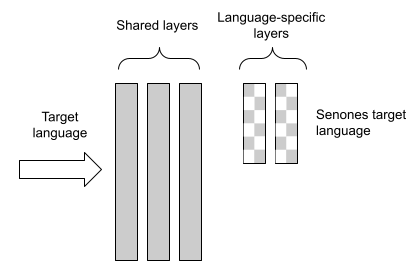
\includegraphics[scale=0.7]{imgs/Ours_final.png}
\caption{Overview of the second step of the Multilingual transfer learning approach. Grey blocks are pre-trained during the multilingual first step. Language-specific layers can be randomly initialized, as indicated by the color white, for a language not present during the multilingual phase or use the corresponding pre-trained layers in case the target language was present during the multilingual training, as indicated by the color grey.}
\label{fig:MLTL1}
\end{center}
\end{figure}


\subsection{Experimental Setup}
\label{section:corpus}
All experiments in this study were conducted using five children corpora, each representing a distinct language: PFSTAR\_SWE, ETLTDE, CMU, LETSREAD, and CHOREC. Detailed descriptions of these datasets are provided in Section \ref{section:children_corpora}. Table \ref{tab:statistics2} offers statistics on the duration, number of speakers, number of utterances and language of each corpus.

% Explain why not Myst 
It is important to note that, in this work, we deliberately focused on utilising small datasets to align with the typical size of available children's speech corpora. Consequently, the MyST children corpus, which is relatively large with over 100 hours of data, was not included in our experiments. Including MyST in this study would introduce a bias toward American English in the multi-task setting, as it represents more than twice the cumulative duration of all our low-resource datasets. While there are ways to mitigate this bias, such as weighting the dataset contributions in the loss function, we chose not to explore this avenue in the scope of this thesis. Our emphasis on smaller datasets aims to better reflect the challenges associated with low-resource scenarios commonly encountered in children's speech research.


%\begin{table}[ht]
%\begin{center}
%\begin{tabular}{llcc}
%\hline
%Corpus name & Language     & Train & Test  \\ \hline
%\multicolumn{1}{l}{PFSTAR\_SWE} & Swedish             & 6030 utt  & 2879 utt  \\ 
%\multicolumn{1}{l}{} &              & 04h00 & 01h48 \\\hline
%\multicolumn{1}{l}{ETLTDE}      & L2 German   & 1445 utt &  339 utt \\ 
%\multicolumn{1}{l}{}      &    &  04h41 & 01h06 \\ \hline
%\multicolumn{1}{l}{CMU}         & English             & 3637 utt & 1543 utt \\ 
%\multicolumn{1}{l}{}         &              & 06h26 & 02h45  \\ \hline
%\multicolumn{1}{l}{LETSREAD}    & Portuguese & 3590 utt & 1039 utt \\ 
%\multicolumn{1}{l}{}    &  & 12h00 & 02h30 \\  \hline
%\multicolumn{1}{l}{CHOREC}      & Dutch               & 2490 utt & 575 utt  \\ 
%\multicolumn{1}{l}{}      &                &  20h12 & 04h42 \\ \hline
%\end{tabular}
%\caption{Statistics on the different corpora of children's speech.}
%\label{tab:statistics2}
%\end{center}
%\end{table}


\begin{table}[]
    \begin{center}

    \begin{tabular}{llcc}
    \hline
    Corpus name                  & Language                                      & Train           & Test            \\ \hline
    \multirow{3}{*}{PFSTAR\_SWE} & \multirow{3}{*}{\textit{Swedish}}             & 6030 utterances & 2879 utterances \\
                                 &                                               & 138 speakers    & 60 speakers     \\
                                 &                                               & 4 hours         & 2 hours         \\ \hline
    \multirow{3}{*}{ETLTDE}      & \multirow{3}{*}{\textit{L2 German}}           & 1445 utterances & 339 utterances  \\
                                 &                                               & 296  speakers   & 72 speakers     \\
                                 &                                               & 5 hours         & 1 hour          \\ \hline
    \multirow{3}{*}{CMU}         & \multirow{3}{*}{\textit{English}}             & 3637 utterances & 1543 utterances \\
                                 &                                               & 76 speakers     & 75 speakers     \\
                                 &                                               & 6 hours         & 3 hours         \\ \hline
    \multirow{3}{*}{LETSREAD}    & \multirow{3}{*}{\textit{European Portuguese}} & 3590 utterances & 1039 utterances \\
                                 &                                               & 180 speakers    & 52 speakers     \\
                                 &                                               & 12 hours        & 2 hours         \\ \hline
    \multirow{3}{*}{CHOREC}      & \multirow{3}{*}{\textit{Dutch}}               & 2490 utterances & 575 utterances  \\
                                 &                                               & 282 speakers    & 70 speakers     \\
                                 &                                               & 20 hours        & 5 hours         \\ \hline
    \end{tabular}
    \caption{Statistics on the different corpora of children's speech.}
\label{tab:statistics2}

\end{center}
    \end{table}

For all experiments in this study, we used the same toolkit, architecture, loss functions and learning rate as in Section \ref{section:exp_setup}. We kept the acoustic model divided into two parts: the first part is shared across all languages, and the second part is language-specific. Given that each corpus represents a distinct language, an independent language model and lexicon are employed for each language. Importantly, these language models and lexicons are kept constant across all experiments in this study, ensuring that any observed changes can be attributed to the acoustic model. Additionally, during the backpropagation process, equal weight contributions are given to all datasets.

%Our experimental design follows the same structure as the previous experiment, as outlined in Section \ref{section:exp_setup}. In this setup, the acoustic model is divided into two parts: the first part is shared across all languages, and the second part is language-specific. As each corpus represent a distinct language, we employ an independent language model and lexicon for each. Importantly, these language models and lexicons remain constant across all experiments to isolate the contribution of the acoustic model. Additionally, during the backpropagation process, all datasets are given equal weight contributions. 

\subsection{Multilingual-transfer learning experiment}

\begin{table*}[ht] 
\begin{center}
\begin{small}
\begin{tabular}{c|ccccc}

\hline
 & PFSTAR\_SWE & ETLTDE & CMU &  LETSREAD & CHOREC   \\  \hline
 \multicolumn{1}{c|}{Language} & \textit{Swedish} & \textit{L2 German}  &  \textit{English}  & \textit{Portuguese} & \textit{Dutch}   \\ \hline
\multicolumn{1}{c|}{Single language} & 54.36\% & 44.69\%  &  21.26\%  & 26.88\% & 25.15\%    \\ \hline
\multicolumn{1}{c|}{MTL} & 54.95\% & 42.46\% & 23.01\% & 27.45\% & 25.10\%   \\ \hline
\multicolumn{1}{c|}{TL from PFSTAR\_SWE} & - & 42.23\% & 20.62\% & 26.47\% & 24.65\%   \\ 
\multicolumn{1}{c|}{TL from  ETLTDE}  & 53.60\% & -  &  20.90\% & 26.61\%  & 25.42\%        \\ 
\multicolumn{1}{c|}{TL from CMU}  & 52.83\%   & 41.54\%    & - & 26.49\% & 24.58\%   \\ 
\multicolumn{1}{c|}{TL from LETSREAD} & 52.50\% & 41.77\%  & 20.41\% & - & 24.60\%   \\ 
\multicolumn{1}{c|}{TL from CHOREC} & 52.20\% & 40.28\%    & 19.77\%    & 26.05\%   & -     \\ \hline
\multicolumn{1}{c|}{TL Average} & 52.78\% & 41.46\% & 20.43\% & 26.41\% & 24.81\%    \\ \hline
\multicolumn{1}{c|}{TL Best} & 52.20\% & 40.28\% & 19.77\% & 26.05\% & 24.58\%    \\ \hline \hline
\multicolumn{1}{c|}{MLTL} & 51.67\% & \textbf{38.04\%} & \textbf{19.33\%} & \textbf{25.75\%} & \textbf{23.78\%}    \\ \hline \hline
\multicolumn{1}{c|}{MLTL-olo}  & \textbf{51.58\%} & 40.05\% & 19.67\% & 26.20\% & 24.57\% \\ \hline


\end{tabular}
\end{small}
\end{center}
\caption{WER results of multilingual-transfer learning and cross-lingual experiments. MTL: Multi-Task Learning, TL: Transfer Learning, MLTL: Multilingual Transfer Learning, MLTL-olo: Multilingual Transfer Learning one-language-out}
\label{tab:result-TL4epoch}
\end{table*}

Table \ref{tab:result-TL4epoch} presents the \ac{WER} results of the \ac{MLTL} approach compared to three different methods: baseline, trained on each corpus individually for 4 epochs; \ac{MTL} alone, trained jointly using all corpora for 4 epochs; \ac{TL} alone, adapted for the target language using, in turn, one of the other 4 baseline models as a source, leading to 4 results per target language. In addition, for clarity, we summarise the transfer learning scores with the average of the 4 scores and the best of the 4 for each target.

Firstly, it is important to emphasise that the baseline scores correctly reflect the different tasks the children were asked to perform and the corresponding amount of data available for each corpus. The best \ac{WER} score, 21.26\% for CMU, can be explained by the reading-aloud-sentences task nature of this corpus. Thus, the language model can more easily compensate for the acoustic model errors. In addition, Chorec and LetsRead, as the largest corpora in our experiment, also yield relatively good results for children's speech recognition. On the other hand, ETLTDE and PFSTAR\_SWE show the worse \ac{WER} results with 44.69\%  and 54.36\% \ac{WER}, respectively. This can be explained by the limited amount of data available and by the language model which does not compensate as much as the CMU model. Especially for ETLTDE, since it is the only corpus that does not contain scripted text, but spontaneous responses. In addition, the age range of PFSTAR\_SWE children also plays a critical role in performance, since younger children generally yield worse performance scores \cite{TFchildren}.

Regarding \ac{MTL}, we observed that this approach did not result in improvements in the baseline performance for almost all languages. This observation aligns with the findings discussed in Section \ref{section:HMMDNNADULT2CHILD}. Nevertheless, we do not observe a significant degradation, suggesting that the model, especially the shared part of the model, is learning shared representations. 

%Turning to multi-task learning, among all the approaches presented, only \ac{MTL} fails to improve the baseline performance for almost all languages, which is in line with our results from Section \ref{section:HMMDNNADULT2CHILD}.  %It can be explained by the differences in terms of the size of the child's speech corpora used. The smaller the size of the corpora used, the more difficult it is to model the acoustic variation in the children's speech.


Concerning \ac{TL}, all performance scores surpass their corresponding baseline, confirming that \ac{TL} is an appropriate method for children's \ac{ASR}. It allows the system to be exposed to an increased amount of children's data in a non-competitive setting like \ac{MTL}. Precisely, Table \ref{tab:result-TL4epoch} indicates that Chorec is the best pre-trained model for knowledge transfer. This aligns with expectations as Chorec is the largest corpus, constituting approximately 40\% of the total data used in our experiments.


Finally, \ac{MLTL} shows an average relative improvement in \ac{WER} of 7.73\%  compared to the baseline, slightly higher than the average (\ac{TL} Avg) and the best (\ac{TL} Best) \ac{TL} performance, with an average relative improvement of 4.50\% and 2.66\%, respectively. 

The strength of \ac{MLTL} is that it can benefit both from \ac{MTL} and \ac{TL}, minimising some of their associated weaknesses.
Attending to our results, \ac{MTL} does not improve single language training. We believe that the unbalanced amount of data, the significant differences among data sets and the use of segmental optimisation (\ac{LF-MMI}) can partially explain these results. This interpretation is further supported by the findings discussed in Section \ref{section:HMMDNNADULT2CHILD}. Nevertheless, we hypothesise that the multi-task objective leans the network towards 
better optimisation of the lower layers, rather than optimising the upper language-specific layers, can still be beneficial for \ac{TL}.
Regarding \ac{TL}, one can observe considerable performance variations depending on the pre-trained model used as the source model, probably due to a poorer initialisation of lower layers that is less efficient for \ac{TL}. The \ac{MLTL} experiments show that we can overcome these drawbacks by combining both \ac{MTL} and \ac{TL}, thus, validating the effectiveness of this approach for robust speech recognition of children.


\subsection{Cross-lingual validation}
\label{section:olo}

In the previous section, we showed that the \ac{MLTL} approach yields better results than separate \ac{MTL} and \ac{TL} frameworks.

To further validate the hypothesis that the shared lower layers are able to learn meaningful information about children's speech characteristics, regardless of the language, we perform a cross-language experiment following a leave one-language-out setting. In this experiment, we keep one language out of the multi-task training and use it only during the \ac{TL} phase to adapt the acoustic model parameters. 

We repeated this procedure for each corpus in our experiment. As in the previous experiment, we used 4 epochs for each learning phase. The last row of Table \ref{tab:result-TL4epoch} presents the results of the cross-language experiment.

For all corpora, the \ac{MLTL-olo} approach outperforms the baseline \ac{WER} score with an average relative improvement of 5.56\%. Improvements are more remarkable for the small corpora ETLTDE and CMU, with a  relative improvement of 14.88\% and 9.07\%, respectively. PFSTAR\_SWE does not benefit as much, with only 5.05\% relative improvement. This is mainly due to the age differences with the children in the other corpora used in the \ac{MTL} phase. Indeed, the children in PFSTAR\_SWE are much younger (see section  \ref{section:children_corpora} for more details). %We hypothesise that these results can be explained by the fact that the shared layers have learned the underlying multilingual features of children's speech.

It is also interesting to compare \ac{MLTL-olo} with the results of transfer learning alone. In both cases, the pre-trained models used have never seen the target language data. We observe that the results between the \ac{MLTL-olo} and \ac{TL} Best are extremely close, with small improvement with the \ac{MLTL-olo}, only the best transfer learning model on LetsRead is slightly better than \ac{MLTL}. This means that during multilingual training the system learned, at least, the best representation of the available children's characteristics. This is consistent with our hypothesis of the important role of the multilingual training phase in our two-step procedure.

\section{Summary and discussion}
%\label{section:conclusions}
In this chapter, we have explored the current state of the art for Hybrid \ac{HMM-DNN} speech recognition systems for children's speech. We aimed to address the following research questions: \textit{Which knowledge transfer approach is best for efficiently modelling and improving traditional automatic recognition of children's speech? Can these approaches be used to efficiently exploit low-resource children's speech data from multiple languages?}

Our results provide a positive response to these questions, first by demonstrating the effectiveness of the knowledge transfer approach for children's \ac{ASR}, especially transfer learning. Particularly, we validated the effectiveness of transfer learning in both English and European Portuguese datasets. This efficacy arises from the ability of transfer learning to efficiently leverage knowledge encapsulated in a source pre-trained model trained on adult speech when applied to the task of training on children's speech. In addition, multi-task learning alone may not yield the most optimal results but we have demonstrated that the shared components of the model have the capacity to learn relevant information across multiple tasks jointly. Offering a trade-off for a multilingual or adult-children \ac{ASR} system. Building upon these insights, this chapter introduces a novel approach—integrating transfer learning and multi-task learning within our multilingual transfer learning system. We demonstrated that the challenges associated with both multi-task and transfer learning can be effectively overcome through the use of our proposed approach. Indeed, this innovative system is built on the strengths of the multi-task learning approach to learn pertinent information jointly, coupled with the efficiency of transfer learning in making effective use of pre-existing knowledge. Even in a low-resource scenario, this approach yielded promising results, resulting in an average relative improvement of 7.73\%. Additionally, the benefits of multilingual pre-training extended to transfer learning with an unseen language, showcasing an average relative improvement of 5.56\%. These findings underscore the suitability of multilingual transfer learning as a robust method for addressing children's speech recognition challenges, particularly in contexts with limited resources.

% Discussion
In the course of this chapter, our primary focus was directed towards the exploration of a multilingual system; however, it is crucial to emphasise the versatility of our approach. Indeed, our methodology could seamlessly be extended to various other tasks beyond multilingual scenarios. This extends to tasks involving age groups, accents, fluency levels, or varying degrees of intelligibility. It is worth noting that we did not extend our investigation to further scenarios within this thesis, primarily due to the limitations of the available datasets. Nonetheless, the extensibility of our approach holds promise for addressing a wide range of challenges across different linguistic and demographic dimensions in future research. In addition, as a future research direction, it would be interesting to investigate the effects of incorporating a larger children's corpus, adult speech corpus or even non-European languages during the multilingual learning phase with specific weighting on the loss. Additionally, understanding how different types of tasks or linguistic variations influence our approach adaptability would be an interesting avenue of research.

% Transition to E2E
In the context of this thesis, we solely employed a \ac{TDNN-F} based architecture within the different \ac{HMM-DNN} systems developed in this chapter. This choice was inspired by earlier research \cite{tdnnf-children} and is acknowledged as the state-of-the-art for children's \ac{ASR} in \ac{HMM}-based systems. However, in response to the emerging use of end-to-end \ac{ASR} and the promising initial results observed for children's \ac{ASR}, a strategic decision was made to transition towards the utilisation of end-to-end systems for the remainder of the thesis. This transition underscores an ongoing commitment to staying abreast of advancements in \ac{ASR} methodologies and exploring innovative approaches that hold the potential to further enhance the recognition accuracy of children's speech.

Finally, it is noteworthy to observe similarities between our approach and the successful XLS-R model \cite{babu2021xlsr}, which is a self-supervised cross-lingual speech representation learning based on wav2vec2 \cite{baevski2020wav2vec}. Similar to our multilingual transfer learning, both approaches use a two-step procedure where a multilingual model is trained first, and then the model is fine-tuned to a specific language/task. While there are differences, such as dataset size and the supervised/unsupervised settings in the first step of training, recognising potential connections and similarities is valuable. It underscores the relevance and potential impact of our approach in the broader landscape of speech representation learning.
